\label{sga}
In his renowned book on Genetic Algorithm David E. Goldberg \citep{Goldberg:89} describes Genetic Algorithms(GA) as search and optimisation technique which is based on the theory of natural selections and natural genetics. These are general search and optimisation algorithms that use the theories behind the evolution as a tool to find optimal or near optimal solution to difficult problems. This involves evolving a population of possible solutions to the particular problem by using operations inspired by natural genetic variation and natural selection \citep{Murphy:03}. 
It simulates the "survival of the fittest" among individual solution over consecutive generation for solving a problem. In 1960's Genetic Algorithms were pioneered by John Holland along with his colleagues and students at University of Michigan\citep{Murphy:03}.

\subsubsection{Optimisation using GA}
In science and Engineering there exist many problems that have solution space too large or sometimes even an infinite set. In those case it is impossible to check each individual solution and try to find the best one. One approach to finding a solution of such problems is limiting the number of possibilities and range with a given step size for lookup. The set of possible solution are known as 'search space'. 

Each possible solution can be marked by its value of fitness for the problem.  Using this fitness value, the algorithm determines which set of solutions are going to forward to produce new solutions. GA attempt to find the best solution based on its fitness value to a given problem. This is achieved by using a combination of \emph{exploitation} and \emph{exploration}. When the algorithm has found a number of good possible solutions it exploits them by combining different parts of each solution to form a new candidate solutions. This is known as \emph{crossover}. GA also do some experiment by creating new candidate solutions by randomly changing parts of old solutions which is known as \emph{mutation}. \citep{Murphy:03}.

In his Master thesis Roderick Murphy described GA as 'weak' optimisation of searching procedure as they do not use any domain specific knowledge to do so\citep{Murphy:03}. Instead GA utilise some 'random' choice to guide its search by exploiting historical information to direct the search into a region of optima.
\subsubsection{GA terminology}
\paragraph{Population:}
Population is a subset of all possible solutions to the given problem.
\paragraph{Chromosome:}
A chromosome is one individual solution to the problem.
\paragraph{Gene:}
A gene is one element position of a chromosome.
\paragraph{Allele:}
Allele is the particular value of a gene in a chromosome.
\paragraph{Locus:}
The position of a gene on the chromosome.
\paragraph{Genotype:}
Genotype is the population in the computation space.
\paragraph{Phenotype:}
Phenotype is the population in the real world solution space.
\citep{Murphy:03}
 
\subsubsection{Computer Implementation}
To utilise GA one must encode solutions to a problem in a structure that can be stored in the computer. A solution to a problem is represented as  string known as \emph{chromosome}(strings) that consist of a combination of several genes(simple representation are binary 1's \& 0's). If we consider a multi-variable problem, a gene can be considered as the bits that encode a particular parameter and its allowable value. A set of solutions to the problem is represented by a group of chromosomes referred to as a \emph{population}. During each iteration of the algorithm the chromosomes in the population will undergo one or more genetic operations such as \emph{crossover} and \emph{mutation}. The result of the genetic operations will become the next generations of the population. This process continues until a solution is found or a certain termination condition is met. \citep{Murphy:03}

\subsubsection{Genetic Operators}
Genetic Operators are responsible for altering the genetic composition of offspring. There three operators:
\begin{itemize}
	\item Selection
	\item Crossover
	\item Mutation
\end{itemize}

\subsubsection{Selection}
Selection operator is used for selecting candidate solutions for reproduction. The probability of selection should be proportional to the fitness value of the chromosome itself. The selection process is very important for maintaining good diversity and preventing premature convergence. There are several methods of how to select the best chromosomes. 

\paragraph{Roulette wheel selection:} In roulette wheel selection parents are selected according to their fitness. The better the fitness value the higher the chances to be selected.
\paragraph{Rank selection:} Rank selection first ranks the population and then every chromosome receives fitness from this ranking. In population with N chromosome, the worst chromosome will have rank 1, second worst  will have 2 and the best one will have N.
\paragraph{Tournament selection:} In Tournament selection K number of individuals are taken from the population then select the best out of these using their fitness value. The process is repeated for selecting next parent.
\citep{tutp.com:98ga}

\subsubsection{Crossover}
The primary purpose of crossover operator is to get genetic material from the previous generation to the next generation. This is done by selecting two parents and then exchanging some parts of their genes. This produces two new offsprings. There are different ways of exchanging genes.
\paragraph{Single-point crossover}
This is the simplest form of crossover in which a random crossover point is selected and the bits from this point get swapped with between two parents to get new offsprings. Figure \ref{fig:sp-cross} demonstrate the the single-point crossover.

\begin{figure}[!htb]
  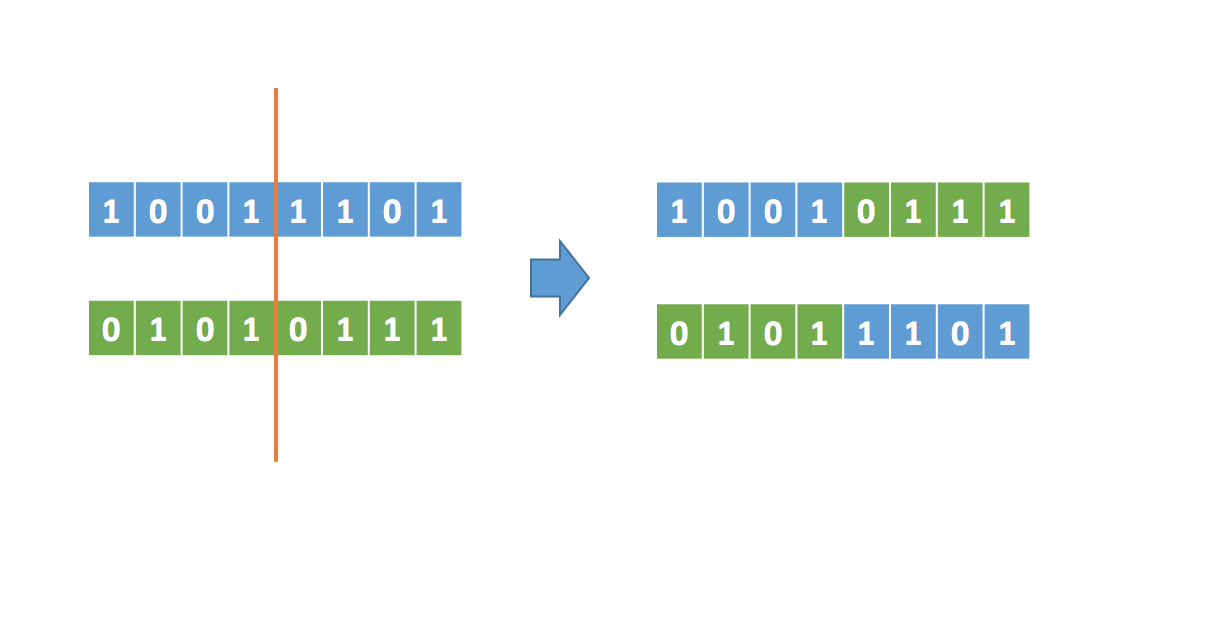
\includegraphics[width=\linewidth]{figs/single-point_crossover.png}
  \caption{Single-point crossover}
  \label{fig:sp-cross}
\end{figure}

\paragraph{Multipoint crossover}
In mulit-point crossover a number of crossover points are chosen and then bits segments in every second group are swapped between two parents to produce new offsprings. Figure \ref{fig:mp-cross} shows multi-point crossover. 

\begin{figure}[!htb]
  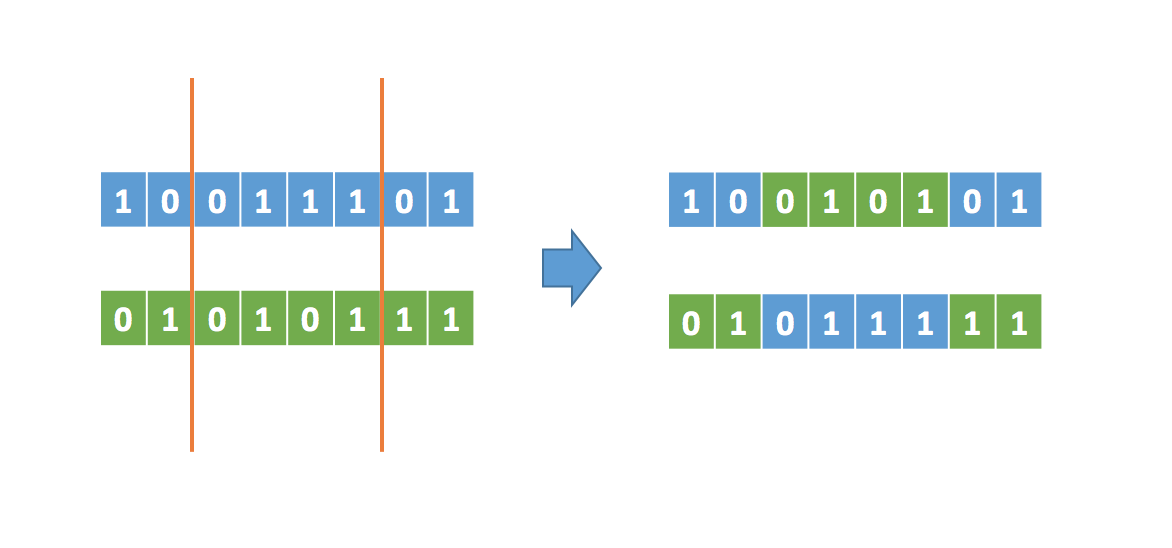
\includegraphics[width=\linewidth]{figs/multi-point_crossover.png}
  \caption{Multi-point crossover}
  \label{fig:mp-cross}
\end{figure}

\paragraph{Uniform crossover}
Uniform crossover is a variation of multi-point crossover. In this method random decision is made whether a bit groups will be swapped or not between two parents to produce new offsprings. Figure \ref{fig:uniform-cross} shows uniform crossover. 

\begin{figure}[!htb]
  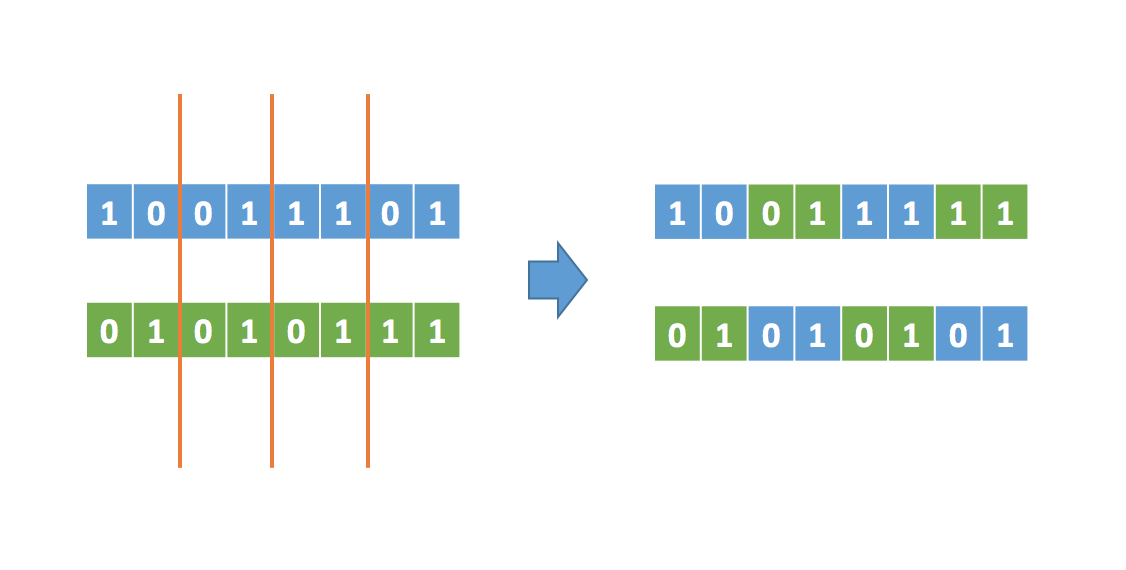
\includegraphics[width=\linewidth]{figs/uniform_crossover.png}
  \caption{Uniform crossover}
  \label{fig:uniform-cross}
\end{figure}
\citep{Murphy:03}

\subsubsection{Mutation}
Mutation operator create new offspring by making small tweak in chromosome. It can help creating chromosomes that would not otherwise be formed by applying selection and crossover operators alone. Mutation can allows GA to explore the search space and keep it from getting trapped in a local optimal solutions. There are several methods of mutation such as bit flipping, random resetting, swap mutation and inversion mutation\citep{tutp.com:98ga}. Figure \ref{fig:mutation} shows bit flipping and Swap mutation.

\begin{figure}[!htb]
  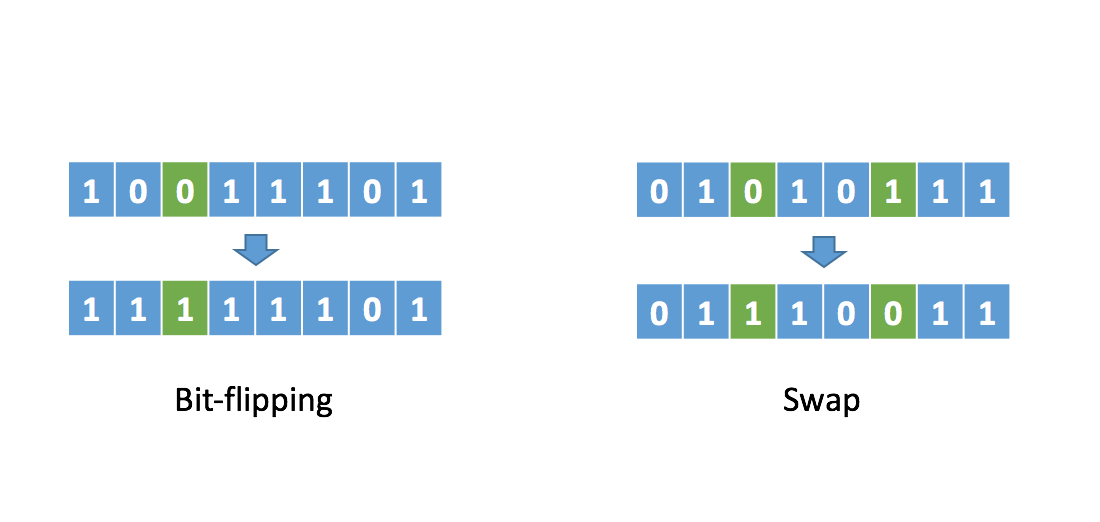
\includegraphics[width=\linewidth]{figs/mutation.png}
  \caption{Mutation}
  \label{fig:mutation}
\end{figure}

\subsubsection{Simple Genetic Algorithm}
\begin{enumerate}
\item \textbf{Start:} Generate random population of n chromosomes (suitable solutions for the problem)
\item \textbf{Fitness:} Evaluate the fitness f(x) of each chromosome x in the population
\item \textbf{New population:} Create a new population by repeating following steps until the new population is complete
	\begin{enumerate}
	\item \textbf{Selection:} Select two parent chromosomes from a population according to their fitness (the better fitness, the bigger chance to be selected)
	\item \textbf{Crossover:} With a crossover probability cross over the parents to form a new offspring (children). If no crossover was performed, offspring is an exact copy of parents.
	\item \textbf{Mutation:} With a mutation probability mutate new offspring at each locus (position in chromosome).
	\item \textbf{Accepting:} Place new offspring in a new population
	\end{enumerate}
\item \textbf{Replace:} Use new generated population for a further run of algorithm
\item \textbf{Test:} If the end condition is satisfied, stop, and return the best solution in current population
\item \textbf{Loop:} Go to step 2
\end{enumerate}
\citep{Obitko:98}

\subsubsection{Application of GA}
Genetics Algorithms are very effective way of quickly finding a reasonable solution to a complex problem. GAs are most effective in search space for which little is known. Apart from general optimisation problems, Genetic Algorithms are successfully deployed on diverse range of other fields. These include tasks optimising, dynamic programming, machine learning, economics, immune systems, ecology, population genetics and social systems. \citep{Murphy:03}


A more recent development is the use of Evolutionary Computation (EC) to evolve the control structures for humanoid robotics \citep{eaton2015}. Writing software in a traditional manner to controls the very large number of articulation points is beyond the capability of a human programmer \citep{eaton2015}. Techniques that leverage GAs have been demonstrated to effectively equip humanoid robotic platforms with abilities to simulate the mechanics of incredibly complex human movement such as kicking a soccer ball.

\subsubsection{Advantages}
Genetic Algorithms have many advantages which inlcude:
\begin{itemize}
\item Does not require any derivative information (which may not be available for many real-world problems).
\item Is faster and more efficient as compared to the traditional methods.
\item Has very good parallel capabilities.
\item Optimizes both continuous and discrete functions and also multi-objective problems.
\item Provides a list of "good" solutions and not just a single solution.
\item Always gets an answer to the problem, which gets better over the time.
\item Useful when the search space is very large and there are a large number of parameters involved.
\end{itemize}

\subsubsection{Limitations}
There are number limitation with Genetic Algorithms that we must consider. These include:
\begin{itemize}
\item GAs are not suited for all problems, especially problems which are simple and for which derivative information is available.

\item Fitness value is calculated repeatedly which might be computationally expensive for some problems.

\item Being stochastic, there are no guarantees on the optimality or the quality of the solution.

\item If not implemented properly, the GA may not converge to the optimal solution
\end{itemize}

\citep{pit:95}

